\documentclass[skript.tex]{subfiles}

\begin{document}
	
	\subsection*{Lebesgue-Maß}
		\begin{enumerate}[(1)]
			\item Für ein verallgemeinertes Integral $I$ der Form
			$(a,b)$, $(a,b]$, $[a,b)$, $[a,b]$ mit \\ $-\infty \leq a \leq b \leq +\infty$ setzen wir
			$\lambda(I) \ceq b-a \in [0,\infty]$
			\item (TODO)
				\stepcounter{cntr} % skip Lemma 30
				\begin{lem}
					\unskip
					Dies ergibt ein eindeutiges $\sigma$-finites Prämaß auf der Algebra $\mc{A}$,
					die aus endlichen Vereinigungen disjunkter Intervalle im obigen Sinne besteht. \\
					Wir setzen
					$\lambda{\left(\bigcupdot_{j=1}^k I_j \right)} = \sum_{j=1}^k \lambda(I_j)$.
				\end{lem}
			\item (TODO) Wir erhalten zunächst eine Fortsetzung von $\lambda$ zu einem äußeren Maß
				$\lambda^*$, also $\lambda^*=\lambda$ auf $\mc{A}$, wobei jede Menge aus
				$\mc{A}$ die Carathéodory-Bedingung erfüllt.
			\item \emph{Satz 28} liefert eine $\sigma$-Algebra $\Lambda\supset\mc{A}$, sodass 
				$\lambda \ceq \lambda^*{\mid_\Lambda}$ ein Maß ist.
			\item
				\begin{defin}
					\unskip
					Die Elemente von $\Lambda$ heißen \textit{Lebesgue-messbare} Mengen (bzw.
					\textit{Lebesgue-Mengen}) und $\lambda$ ist das \textit{Lebesgue-Maß}.
				\end{defin}
		\end{enumerate}
		
		\addtocounter{cntr}{-3} % add left-out Lemma
		\begin{lem}[Ad 3]
			Sei $\mu$ ein Prämaß auf einer Algebra $\mc{A} \sbs \mf{P}(X)$. \\
			Wir setzen für $A \sbs X$
			\[
				\mu^*(A) = \inf\left\{ 
				  \sum_{k\in\N} \mu(A_k)
				  \Bigm\vert (A_k)_{k\in\N} \sbs A, A \sbs \bigcup_{k\in\N} A_k
				\right\}
			\]
			Dies definiert ein äußeres Maß $\mu^*$ mit $\mu^* = \mu$ auf $\mc{A}$
			und jede Menge aus $\mc{A}$ erfüllt die Carathéodory-Bedingung. % TODO: Overfull hbox
		\end{lem}
		\addtocounter{cntr}{2} % return to normal counting
		
		\begin{proof}
			\hfill\\ % TODO: Not beautiful at all...
			\emph{1. Teil:} Übungsaufgabe 5. \\
			\emph{2. Teil: (Carathéodory-Eigenschaft):}\quad
			Sei $E \sbs X$ beliebig und $A \sbs \mc{A}$. \\
			(Ziel: $\mu^*(E) \geq \mu^*(E \cap \cp{A}) + \mu^*(E \cap A)$, ''$\leq$'' folgt sofort aus der Subadditivität).
			
			Wir betrachten eine beliebige Überdeckung von $E$ durch
			\[
				(B_k)_{k\in\N} \sbs \mc{A},\quad B \ceq \bigcup_{k\in\N} B_k \supset E.
			\]
			Dann ist zunächst auch $(B_k \cap A)_{k\in\N}$ eine Überdeckung von $E \cap A$
			und entsprechend \\ $(B_k \cap \cp{A})_{k\in\N}$ eine Überdeckung von $E \cap \cp{A}$.
			
			Wir erhalten hieraus
			\[
				\sum_{k\in\N} \mu(B_k) = \sum_{k\in\N} \mu(B_k \cap A) 
									+ \sum_{k\in\N} \mu(B_k \cap \cp{A})
					\geq \mu^*(E \cap A) + \mu^*(E \cap \cp{A})
			\]
			Indem wir das Infimum über $(B_k)_{k\in\N}$ mit $\bigcup_{k\in\N} B_k \supset E$ nehmen,
			folgt 
			\[
				\mu^*(E) \geq \mu^*(E \cap A) + \mu^*(E \cap \cp{A}).
			\]
		\end{proof}
		
		Dies erledigt (3). Für (2) erbringen wir
		\begin{proof}[Beweis von Lemma 31]
			\hfill % TODO: Not beautiful at all...
			\begin{enumerate}[(a)]
				\item \emph{$\mc{A}$ ist eine Algebra}.\quad In der Tat, $\mbb{R} = (-\infty,\infty)$.
					Das Komplement einer endlichen Vereinigung disjunkter Intervalle
					(möglicherweise verallgemeinert) besitzt wieder diese Form.
					
					Für den Fall endlicher Vereinigungen betrachte zunächst den Fall zweier aus je
					einem Intervall bestehender Mengen ($\rightarrow$ entweder disjunkte
					Vereinigung oder neues Intervall) und fahre induktiv fort.
				\item Offenbar gilt $\lambda(\es) = 0$. Für $\sigma$-Additivität ist
					$\lambda(\bigcup_{k\in\N} I_k) = \sum_{k\in\N} \lambda(I_k)$ für alle paarweise
					disjunkten Folgen $(I_k)_{k\in\N} \sbs \mc{A}$ zu zeigen.
					
					\begin{itemize}
						\item Weil jedes $I_k$ eine endliche Vereinigung disjunkter Intervalle ist,
							können wir umsortieren und umnummerieren und somit ohne
							Einschränkungen voraussetzen, dass jedes $I_k$ ein Intervall ist
							(Nach wie vor $(I_k)_{k\in\N}$ paarweise disjunkt).
						\item Weiter können wir voraussetzen, dass $I \ceq \bigcup_{k\in\N} I_k$
							($=$ disjunkte Vereinigung endlich vieler Intervalle, da $\in \mc{A}$)
							aus genau einem Intervall besteht (betrachte jede Komponente der
							Vereinigung separat).
					\end{itemize}
					Wir haben erreicht:
					\addtocounter{footnote}{-2}
					\[
						\sum_{j=1}^\infty \lambda(I_j) \longleftarrow \sum_{j=1}^k \lambda(I_j)
						\darrow{\text{Add.}}{=} \lambda{\Bigg( \bigcup_{j=1}^k I_j \Bigg)}
						\darrow{\text{Monot.}\footnotemark}{\leq}
						\lambda{\Bigg( \bigcup_{j=1}^\infty I_j \Bigg)} = \lambda(I)
					\]
					\footnotetext[10]{$\lambda{\left(\bigcup_{j=1}^k B_j\right)}
								= \sum_{j\in\N}^k \lambda(B_j)$
								vgl. Beweis zu \emph{Satz 12(i)}.}
					Für die andere Richtung wählen wir zunächst für jedes $k\in\N$ ein 
					\emph{offenes} $J_k \supset I_k$ mit
					\[
						\lambda(J_k) \leq \lambda(I_k) + \frac{\epsilon}{2^k}
					\]
					für ein zu bestimmendes $\epsilon > 0$.
					
					Sei zunächst $I$ kompakt. Dann können wir endlich viele $J_k$ auswählen,
					sodass diese $I$ überdecken\footnote[11]{Satz von Heine-Borel}.
					Wir können durch Umnummerierung erreichen, dass dies die ersten $K$ Elemente 
					sind und wir haben
					%\addtocounter{footnote}{-3}
					\[	
						\lambda(I) \overset{\text{Monot.}\footnotemark[10]}{\leq}
						\lambda{\Bigg(\bigcup_{j=1}^K J_j\Bigg)} \overset{\text{Subadd.}}{\leq}
						\sum_{j=1}^K \lambda(J_j)  \overset{\text{Konstr.}}{\leq}
						\epsilon + \sum_{j=1}^K \lambda(I)
					\]
					%\addtocounter{footnote}{1}
					Mit $\epsilon \searr 0$ folgt $\sigma$-Additivität für kompakte $I$.
					Da wir mit Additivität und \\ $\lambda(\{x\}) = \lambda([x,x]) = 0 \ 
					\forall x \in \mbb{R}$ Endpunkte an Intervalle hinzufügen / entfernen können,
					folgt die Behauptung auch für beschränkte $I$.
					
					Sei $I$ nun ein unbeschränktes Intervall, damit ist $\lambda(I) = \infty$. \\
					Zu zeigen ist, $\sum_{j=1}^\infty \lambda(I_j) = \infty$. \\
					Sei $\xi \in I$. Durch Hinzufügen eines Punktes (sofern erforderlich) können wir
					erreichen, dass $I$ abgeschlossen ist. Damit ist $I \cap [-x,x]$ kompakt für jedes
					$x \in \mbb{R}$ und wird folglich von den ersten $K$ Elementen überdeckt,
					$K = K(\xi)$.
					
					Demnach erhalten wir
					\[
						\sum_{j=1}^\infty \lambda(I_j) \geq \sum_{j=1}^K \lambda(I_j)
						 \overset{\text{Konstr. } J_k}{\geq} \left(\sum_{j=1}^K \lambda(J_j)\right)
						 -\epsilon \overset{\text{s.\,o.}}{\geq} \lambda(I \cap [-x,x]) -\epsilon
						 \geq x - \lvert\xi\rvert - \epsilon
					\]
					Hieraus folgt
					\[
						\sum_{j=1}^\infty \lambda(I_j) \geq x - \lvert\xi\rvert - \epsilon
						\xrightarrow{x \to \infty} \infty.
					\]
			\end{enumerate}
		\end{proof}
			
		\begin{minipage}[t]{0.4\textwidth}
			\textbf{Riemann-Integral} \\
			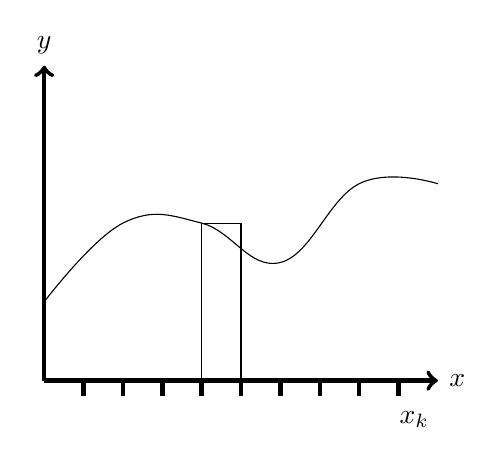
\begin{tikzpicture}
				\draw[->,ultra thick] (0,0)--(5,0) node[right]{$x$};
				\draw[->,ultra thick] (0,0)--(0,4) node[above]{$y$};
				\draw plot [smooth, tension = .7] coordinates {(0,1) (1,2) (2,2) (3,1.5) (4,2.5) (5,2.5)};
				
				\foreach \x in {1,...,9}
				{
					\draw[ultra thick] (\x/2,0)--(\x/2,-.2);
				}
				\node at (4.7,-.5) {$x_k$};
				\draw (2,2) rectangle (2.5,0);
				
			\end{tikzpicture}
			\[
				\int f \approx \sum_{j=1}^k (x_j-x_{j-1}) f(x_j)
			\]
			Kriterium \\
			$($Obersumme $-$ Untersumme$)$ $ \to 0$ 
			
			\medskip
			$f$ muss hinreichend „schön“ sein (z.\,B. nicht überabzählbar viele Sprünge). \\
			z.\,B. nicht Riemann-integrierbar: $\rchi_\mbb{Q}$
		\end{minipage}
		\hfill
		\begin{minipage}[t]{0.4\textwidth}
			\textbf{Lebesgue-Integral} \\
			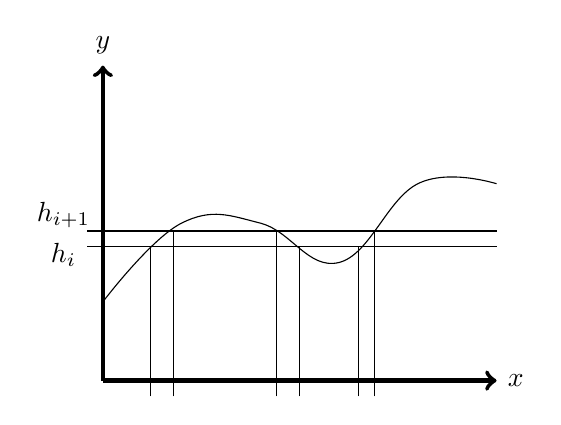
\begin{tikzpicture}
				\draw[->,ultra thick] (0,0)--(5,0) node[right]{$x$};
				\draw[->,ultra thick] (0,0)--(0,4) node[above]{$y$};
				\draw plot [smooth, tension = .7] coordinates {(0,1) (1,2) (2,2) (3,1.5) (4,2.5) (5,2.5)};
				
				\draw (-.2,1.9)--(5,1.9);
				\draw (-.2,1.7)--(5,1.7);
				
				\draw (.6,-.2)--(.6,1.7);
				\draw (.9,-.2)--(.9,1.9);
				
				\draw (2.5,-.2)--(2.5,1.7);
				\draw (2.2,-.2)--(2.2,1.9);
				
				\draw (3.25,-.2)--(3.25,1.7);
				\draw (3.45,-.2)--(3.45,1.9);
				
				\node at (-.5,2.1) {$h_{i+1}$};
				\node at (-.5,1.6) {$h_i$};
				
			\end{tikzpicture}
			\[
				\int f \approx \sum_{k\in\N} h_k\ \lambda\Big(f^{-1}\big([h_k,h_{k+1}]\big)\Big)
			\]
			Hierfür müssen die Urbilder der Intervalle messbar sein.
		\end{minipage}
		
		\section{Messbare Funktionen}
		
		\begin{defin}
			Seien $(X,\Sigma_X)$, $(Y,\Sigma_Y)$ Messräume.Eine Funktion $f \colon X \to Y$ heißt \textit{messbar} (eigentlich \textit{$\Sigma_X$-$\Sigma_Y$-messbar}), falls $f^{-1}(A) \in \Sigma_X\: \forall A \in \Sigma_Y$.
				
			Ist $X$ ein topologischer Raum und $\Sigma_X$ die entsprechende
			Borel-$\sigma$-Algebra, so nennen wir eine messbare Funktion
			\textit{Borel-Funktion}.
		\end{defin}
		
		\begin{bem}
			Es genügt, Messbarkeit für ein Messystem $S \sbs \mf{P}(Y)$ mit $\Sigma(S) = \Sigma_Y$
			zu überprüfen.
			
			In der Tat ist $f^{-1}(A) \in \Sigma_X$ für jedes $A \in S$, es folgt
			\[
				f^{-1}(\cp{A}) = f^{-1}(Y \sm A) = X \sm f^{-1}(A) 
				= \cp{\big(f^{-1}(A)\big)} \in \Sigma_X.
			\]
			Weiter ist
			\[
				f^{-1}{\Bigg( \bigcup_{k\in\N} A_k \Bigg) 
				= \bigcup_{k\in\N} \underbrace{f^{-1}(A_k)}_{\mathrlap{\in \Sigma_X}}
				\in \Sigma_X}.
			\]
		\end{bem}
	
		\setcounter{footnote}{11}


		
\end{document}